%
% SECTION: The tool
%
\section{The tool}
\begin{frame}
  \frametitle{Summary}
  \tableofcontents[currentsection, hideothersubsections]
\end{frame}
\subsection{Architecture}
\begin{frame}
  \frametitle{}
  \framesubtitle{}
  \begin{center}
    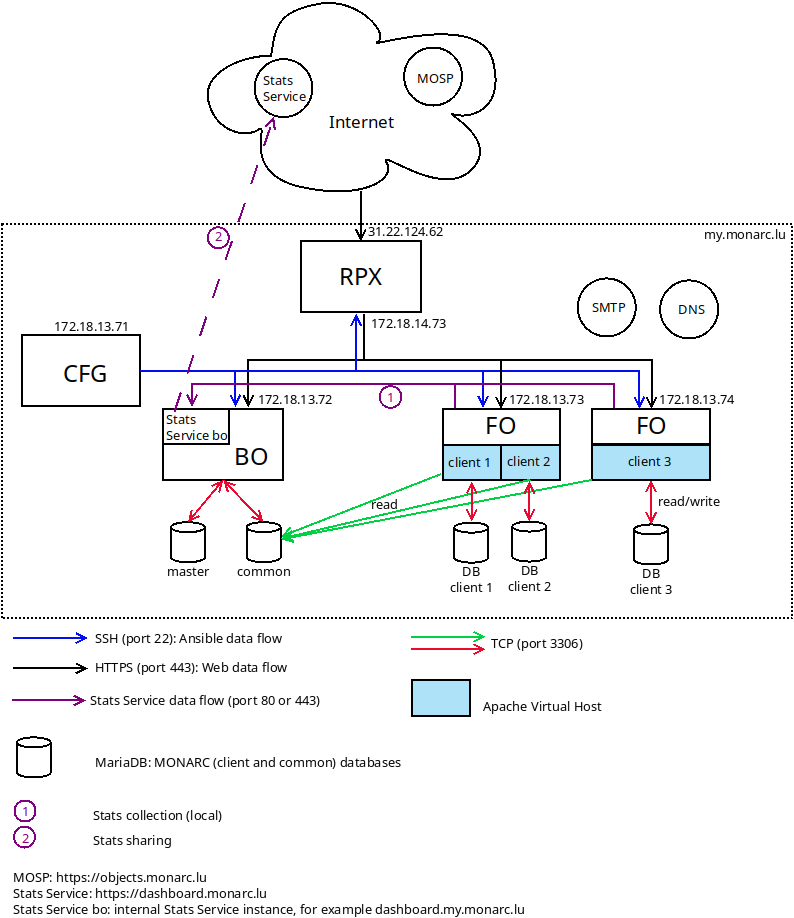
\includegraphics[scale=0.26]{pictures/monarc-architecture.png}
  \end{center}
\end{frame}



\subsection{Workshop}
\begin{frame}
  \frametitle{Le'ts work a little!}
  \framesubtitle{}
  \begin{itemize}
    \item training instance: \url{https://formation.monarc.lu}
    \item login: \texttt{user\_X@monarc.lu}, where $01 \leq X \leq 30$;
    \item password: \texttt{Password1234!}
  \end{itemize}

  \bigskip

  or use the virtual machine: \url{https://vm.monarc.lu}

  \bigskip
  Compatible Web browsers: Firefox, Chrome and Safari.
\end{frame}



\subsection{Modules}
\subsubsection{Dashboard}
\begin{frame}
  \frametitle{Dashboard}
  \framesubtitle{}
  \begin{itemize}
    \item provide different visualizations of the current analysis state;
    \item visualizations are exportable (.png, .csv, .pptx).
  \end{itemize}
\end{frame}

\subsubsection{Statement of Applicabitity}
\begin{frame}
  \frametitle{Statement of Applicabitity}
  \framesubtitle{}
  Statement of Applicability (SOA) and compliance level for a referential security.
\end{frame}

\subsubsection{Record of processing activities}
\begin{frame}
  \frametitle{Record of processing activities}
  \framesubtitle{}
  Register of the information treatment for processing activities.
\end{frame}



\subsection{Roadmap}
\subsubsection{Past}
\begin{frame}
  \frametitle{Latest notable developments}
  \framesubtitle{}
  \begin{itemize}
    \item definition of custom scales for operational risks
      (\href{https://www.monarc.lu/news/2021/09/02/monarc-2110-released/}{MONARC 2.11.0});
    \item dashboard for the CEO with data gathered from different MONARC instances
      (\href{https://www.monarc.lu/news/2020/12/18/monarc-2101-released/}{MONARC 2.10.1});
    \item records of processing activities for the GDPR and set of recommendations
      (\href{https://www.monarc.lu/news/2019/08/23/monarc-290-released/}{MONARC 2.9.0});
    \item connection with MOSP
      (\href{https://www.monarc.lu/news/2019/05/28/monarc-282-released/}{MONARC 2.8.2});
    \item statement of applicability
      (\href{https://www.monarc.lu/news/2018/08/22/monarc-270-released/}{MONARC 2.7.0}).
  \end{itemize}
\end{frame}

\subsubsection{Future}
\begin{frame}
  \frametitle{Future developments}
  \framesubtitle{}
  \begin{itemize}
    \item enhancements to the global dashboard towards a
    security weather forecast\footnote{\url{https://dashboard.monarc.lu}};
    \item enhancements to the sharing of MONARC objects with
    MOSP\footnote{\url{https://objects.monarc.lu}};
    \item import of models in back office;
    \item link between GDPR module and some objects in MONARC.
  \end{itemize}
  \bigskip
  Idea ?
  $\rightarrow$
  \href{https://github.com/monarc-project/MonarcAppFO/issues/new?labels=feature+request}{Feature request}
\end{frame}
